\section{Results and Analysis}
\label{sec:results}

The performance of the proposed morphological tokenizer was evaluated using the TR-MMLU benchmark dataset, which comprises over 1.6 million characters and approximately 200,000 words curated specifically for Turkish \cite{bayram_setting_2025}. This dataset is designed to reflect the linguistic complexity of Turkish, including its rich morphology, agglutinative structures, and diverse syntactic constructions. As such, it provides a rigorous basis for assessing tokenization quality in morphologically complex languages.

The evaluation compared different tokenizers. Each tokenizer was assessed using a consistent set of linguistic and computational metrics introduced in \cite{bayram_tokenization_2025}. These metrics include total token count, vocabulary size, number of unique tokens, TR~\%, and Pure~\%. TR~\% quantifies the proportion of tokens that correspond to valid Turkish words or morphemes, while Pure~\% measures the proportion of tokens that fully align with unambiguous root or affix boundaries, thus reflecting morphological integrity. Importantly, TR~\% and Pure~\% are computed using an independent morphological validator with curated lexical resources external to the tokenizer under evaluation, following the protocol of \cite{bayram_tokenization_2025}, which ensures fair comparison and avoids circularity.

\begin{table}[H]
\centering
\caption{Performance of the proposed TurkishTokenizer on the TR-MMLU dataset.}
\label{tab:turkish_tokenizer_results}
\begin{tabular}{|l|c|}
\hline
\rowcolor[HTML]{DDDDDD}
\textbf{Metric} & \textbf{Value} \\ \hline
Vocabulary Size & 32,768 \\ \hline
Total Token Count & 707,727 \\ \hline
Processing Time (s) & 0.6714 \\ \hline
Unique Token Count & 11,144 \\ \hline
Turkish Token Count & 10,062 \\ \hline
TR~\% & 90.29\% \\ \hline
Pure Token Count & 9,562 \\ \hline
Pure~\% & 85.80\% \\ \hline
\end{tabular}
\end{table}

Despite employing significantly smaller vocabulary sizes, the proposed tokenizer demonstrated better linguistic segmentation. With a vocabulary of 32,768 tokens and 11,144 unique tokens used during evaluation, it balanced generalization and expressiveness more effectively than models such as \texttt{gemma-2-9b} and \texttt{aya-expanse}, which rely on vocabularies of over 255,000 tokens. These large-vocabulary tokenizers, rooted in frequency-based subword segmentation, tend to fragment morphologically rich expressions and introduce ambiguity in downstream tasks. In contrast, the morphological awareness of TurkishTokenizer enables semantically coherent token formation and more consistent syntactic parsing.

Although the total token count generated by the proposed tokenizer (707,727) exceeds those of the other models-for instance, \texttt{aya-expanse} produced 434,526 tokens-this increase is offset by gains in interpretability and linguistic fidelity. High TR~\% and Pure~\% scores suggest reduced reliance on spurious subword splits and improved preservation of morphosyntactic structure.

These findings support the hypothesis introduced in \cite{bayram_tokenization_2025}, which argues that high linguistic alignment in tokenization correlates strongly with downstream model performance. While conventional subword tokenizers may suffice for high-resource languages like English, they exhibit clear limitations in Turkish unless informed by morphological structure. The results presented here highlight the effectiveness of combining rule-based linguistic analysis with subword strategies to produce tokenizers that are both accurate and efficient in morphologically complex settings.

To illustrate the linguistic fidelity of different tokenization strategies, we present a qualitative comparison using the Turkish sentence:

\textit{"Atasözleri geçmişten günümüze kadar ulaşan anlamı bakımından mecazlı bir mana kazanan kalıplaşmış sözlerdir."} \\
(“Proverbs are fixed expressions passed down from the past to the present that acquire a metaphorical meaning in terms of their significance.”)

This sentence contains a wide range of morphological features, including compound words, multiple derivational and inflectional suffixes, and root forms that undergo phonological alternations. These properties make it an ideal test case for evaluating the morphological sensitivity of different tokenizers.

\vspace{1em}

\textbf{Proposed TurkishTokenizer:} \\
The proposed tokenizer segments the sentence into linguistically meaningful units with high fidelity. It produces:
\tokseq{["<uppercase>", " atasöz", "leri", " geçmiş", "ten", " gün", "üm", "üz", "e", " kadar", " ulaş", "an", " anlam", "ı", " bakım", "ın", "dan", " mecaz", "lı", " bir", " mana", " kazan", "an", " kalıp", "laş", "mış", " söz", "ler", "dir", "."]}
It correctly separates suffixes such as (\texttt{"ın", "dan", "lı", "an", "mış", "dir"}), extracts root forms such as \texttt{"atasöz", "gün", "mana"} with leading spaces to mark word boundaries, and employs the \texttt{"<uppercase>"} token to preserve orthographic case.

\vspace{1em}

\textbf{Mursit tokenizer:} \\
The Mursit tokenizer~\cite{mecellem2026} tends to preserve frequent surface forms as whole tokens rather than isolating productive suffix boundaries. It produces:
\tokseq{["At", "asöz", "leri", " geçmişten", " günümüze", " kadar", " ulaşan", " anlamı", " bakımından", " mec", "azlı", " bir", " man", "a", " kazanan", " kalıp", "laşmış", " söz", "lerdir", "."]}
Compared with TurkishTokenizer, it splits the compound root \texttt{"atasöz"} into \texttt{"At", "asöz"} and keeps long inflected spans such as \texttt{"geçmişten"}, \texttt{"günümüze"}, \texttt{"ulaşan"}, and \texttt{"lerdir"} intact, which reduces morpheme-level interpretability.

\vspace{1em}

\textbf{CosmosGPT2 tokenizer:} \\
The CosmosGPT2 tokenizer~\cite{kesgin2024introducing} behaves similarly, but fragments some roots even more aggressively into smaller BPE pieces. It produces:
\tokseq{["At", "as", "öz", "leri", " geçmişten", " günümüze", " kadar", " ulaşan", " anlamı", " bakımından", " mec", "az", "lı", " bir", " man", "a", " kazanan", " kalıp", "laşmış", " söz", "lerdir", "."]}
It breaks \texttt{"atasözleri"} into three root fragments (\texttt{"At", "as", "öz"}) and still keeps many inflected spans unanalyzed, so both lexical integrity and suffix transparency are weaker than in TurkishTokenizer.

\vspace{1em}

\textbf{Tabi tokenizer:} \\
The Tabi tokenizer, used here as the tokenizer component of TabiBERT~\cite{turker_tabibert_2026}, applies coarse merges that often retain whitespace-attached spans as single units. It produces:
\tokseq{["A", "tasöz", "leri ", "geçmişten ", "günümüze kadar ", "ulaşan ", "anlamı ", "bakımından ", "mec", "az", "lı bir ", "mana ", "kazanan ", "kalıp", "laşmış", " söz", "lerdir", "."]}
This behavior obscures internal morphology even more strongly: the root \texttt{"atasöz"} is split into \texttt{"A", "tasöz"}, several tokens absorb following spaces, and multiword or inflected spans such as \texttt{"günümüze kadar "} are preserved as opaque units.

\vspace{1em}

\textbf{Gemma-3:} \\
The tokenizer \texttt{google/gemma-3} segments the sentence as: \\
\tokseq{["<bos>", "At", "as", "öz", "leri", " geçmiş", "ten", " gün", "ümü", "ze", " kadar", " ulaş", "an", " anlam", "ı", " bakım", "ından", " mec", "az", "lı", " bir", " mana", " kaz", "anan", " kal", "ı", "pla", "ş", "mış", " söz", "lerdir", "."]}
Although it captures some suffixes like \texttt{"ten"} and \texttt{"ından"}, it fragments common roots (\texttt{"At", "as", "öz"} instead of \texttt{"atasöz"}) and fails to isolate inner morphemes in forms such as \texttt{"lerdir"} and \texttt{"kazanan"}, limiting morphological interpretability.

\vspace{1em}

\textbf{YTU (Yıldız Technical University) Turkish GPT-2 (without pruned vocab to 32k):} \\
The tokenizer \texttt{ytu-ce-cosmos/turkish-gpt2-large-750m-instruct-v0.1}, trained on Turkish corpora, yields: \\
\tokseq{["At", "as", "öz", "leri", " geçmişten", " günümüze", " kadar", " ulaşan", " anlamı", " bakımından", " mec", "az", "lı", " bir", " mana", " kazanan", " kalıp", "laşmış", " söz", "lerdir", "."]}
Although it still segments \texttt{"atasözleri"} incorrectly, it performs well with forms like \texttt{"geçmişten"}, \texttt{"günümüze"}, and \texttt{"bakımından"}, showing the advantage of Turkish-specific pretraining.

\vspace{1em}

\textbf{GPT-4o:} \\
The tokenizer \texttt{gpt-4o-o200k\_base} generates: \\
\tokseq{["At", "as", "öz", "leri", " geçmiş", "ten", " gün", "ümü", "ze", " kadar", " ulaş", "an", " anlam", "ı", " bakım", "ından", " mec", "az", "lı", " bir", " mana", " kaz", "anan", " kal", "ı", "pla", "ş", "mış", " söz", "ler", "dir", "."]}
Its segmentation strategy is aware of Turkish morphemes but limited by frequent over-segmentation of compound and derived forms.

\vspace{1em}

The results presented in this section provide strong empirical support for the hypothesis introduced in the introduction: tokenizers that explicitly incorporate morphological and phonological knowledge of Turkish can outperform general-purpose models in both segmentation accuracy and linguistic coherence. While most state-of-the-art tokenizers struggle with root-fragmentation, over-segmentation, and inconsistent affix treatment, the proposed hybrid tokenizer consistently identifies morpheme boundaries, preserves semantically meaningful units, and reduces vocabulary redundancy. These findings validate the motivation behind this work: morphologically informed tokenization is essential for robust and interpretable NLP in agglutinative languages like Turkish. The qualitative comparisons presented here illustrate not only the performance gap between general and language-specific tokenizers, but also the need for tokenizer architectures that respect language-internal rules.

\textbf{Downstream Task Evaluation.}

To assess the impact of morphologically informed tokenization on downstream model performance, we evaluated the embeddings produced by models initialized with different tokenizers using three benchmarks: STSb-TR, TR-MTEB~\cite{baysan-gungor-2025-tr}, and TurBLiMP. All models were initialized randomly to isolate the effect of tokenization structure from pre-training data.

Concretely, we construct four sentence embedding models that share the same encoder architecture (\texttt{google/embeddinggemma-300m}; EmbeddingGemma~\cite{vera_embeddinggemma_2025}) and vocabulary size (32,768). Each model is randomly initialized with a fixed seed (42) and trained under an identical embedding-distillation objective against a teacher embedding model based on the same architecture.\footnote{\url{https://huggingface.co/google/embeddinggemma-300m}} The only difference between models is the tokenizer used to produce the token ID sequences. We refer to these models as \texttt{*-random} to emphasize that they start from random weights rather than a pretrained checkpoint, so downstream differences primarily reflect inductive bias introduced by tokenization and decoding choices under a controlled training budget.

Training data comes from a Turkish text corpus with pre-computed teacher embeddings.\footnote{\url{https://huggingface.co/datasets/alibayram/cosmos-corpus-0-05-with-embeddings}} We additionally prepare a unified encoded dataset that stores token ID sequences for all compared tokenizers.\footnote{\url{https://huggingface.co/datasets/alibayram/cosmos-corpus-encoded}} To ensure an apples-to-apples comparison under a fixed context window, we discard any sample for which \emph{any} tokenizer produces a sequence longer than 2048 tokens, so that no model benefits from truncation artifacts or sees different content due to length differences.

TurkishTokenizer is released as a Hugging Face-compatible tokenizer (loadable via \texttt{AutoTokenizer.from\_pretrained} with \texttt{trust\_remote\_code=True}).\footnote{\url{https://huggingface.co/alibayram/turkish-mft-tokenizer}} This allows the same \texttt{sentence-transformers} training and evaluation stack to consume all tokenizers through a standard interface. For large-scale preprocessing, we additionally provide a high-performance Rust-backed implementation as a Python Package Index (PyPI) package.\footnote{\url{https://pypi.org/project/turkish-tokenizer/}}

\begin{table}[H]
\centering
\caption{Embedding distillation experiment setup.}
\label{tab:distillation_setup}
\begin{tabular}{ll}
\toprule
\textbf{Component} & \textbf{Specification} \\
\midrule
Student architecture & \texttt{google/embeddinggemma-300m} (SentenceTransformer) \\
Initialization & Random weights with fixed seed; vocab resized to 32,768 \\
Training objective & Cosine embedding loss against teacher vectors \\
Teacher model & EmbeddingGemma-300M \\
Training corpus & Cosmos corpus with teacher embeddings \\
Training dataset & Unified encoded corpus (4 token streams) \\
Context length & 2048; samples dropped if any tokenizer exceeds the limit \\
Batch size / learning rate & 256 / $5 \times 10^{-5}$ \\
Schedule & Two-phase: 100-step warmup then 1 full epoch \\
Precision & bfloat16 (BF16); gradient checkpointing enabled \\
Hardware & NVIDIA H100 80GB (single node) \\
\bottomrule
\end{tabular}
\end{table}

For STS, we use the Turkish STSb-TR benchmark consisting of sentence pairs with human similarity ratings on a 0--5 scale \cite{beken_fikri_semantic_2021}.\footnote{\url{https://huggingface.co/datasets/figenfikri/stsb_tr}} Each model encodes both sentences, we compute cosine similarity between the resulting sentence embeddings, and we report Pearson and Spearman correlation with the normalized gold scores. Throughout this section, correlations are presented as percentages ($\times 100$) for readability.

We evaluated the models on the Turkish STS benchmark (stsb-tr) without task-specific fine-tuning. Results are summarized in Table~\ref{tab:sts_results}. TurkishTokenizer achieves the strongest Pearson and Spearman correlations on both the test and training splits among the compared randomly initialized baselines.

\begin{table}[H]
\centering
\caption{STS benchmark correlations across train and test splits.}
\label{tab:sts_results}
\begin{tabular}{llrr}
\toprule
\textbf{Model} & \textbf{Split} & \textbf{Pearson} & \textbf{Spearman} \\
\midrule
TurkishTokenizer & test & \textbf{51.44} & \textbf{50.03} \\
Mursit & test & 46.63 & 45.72 \\
CosmosGPT2 & test & 43.09 & 42.18 \\
Tabi & test & 43.01 & 42.53 \\
\midrule
TurkishTokenizer & train & \textbf{54.76} & \textbf{51.90} \\
Mursit & train & 48.99 & 46.93 \\
CosmosGPT2 & train & 44.47 & 43.34 \\
Tabi & train & 45.06 & 43.80 \\
\bottomrule
\end{tabular}
\end{table}

To better understand the learning dynamics, we analyzed the performance evolution of each model across different training checkpoints. Figure \ref{fig:version_history_pearson} shows Pearson correlation across model revisions. The x-axis represents sequential checkpoints ordered by timestamp.

\begin{figure}[H]
    \centering
    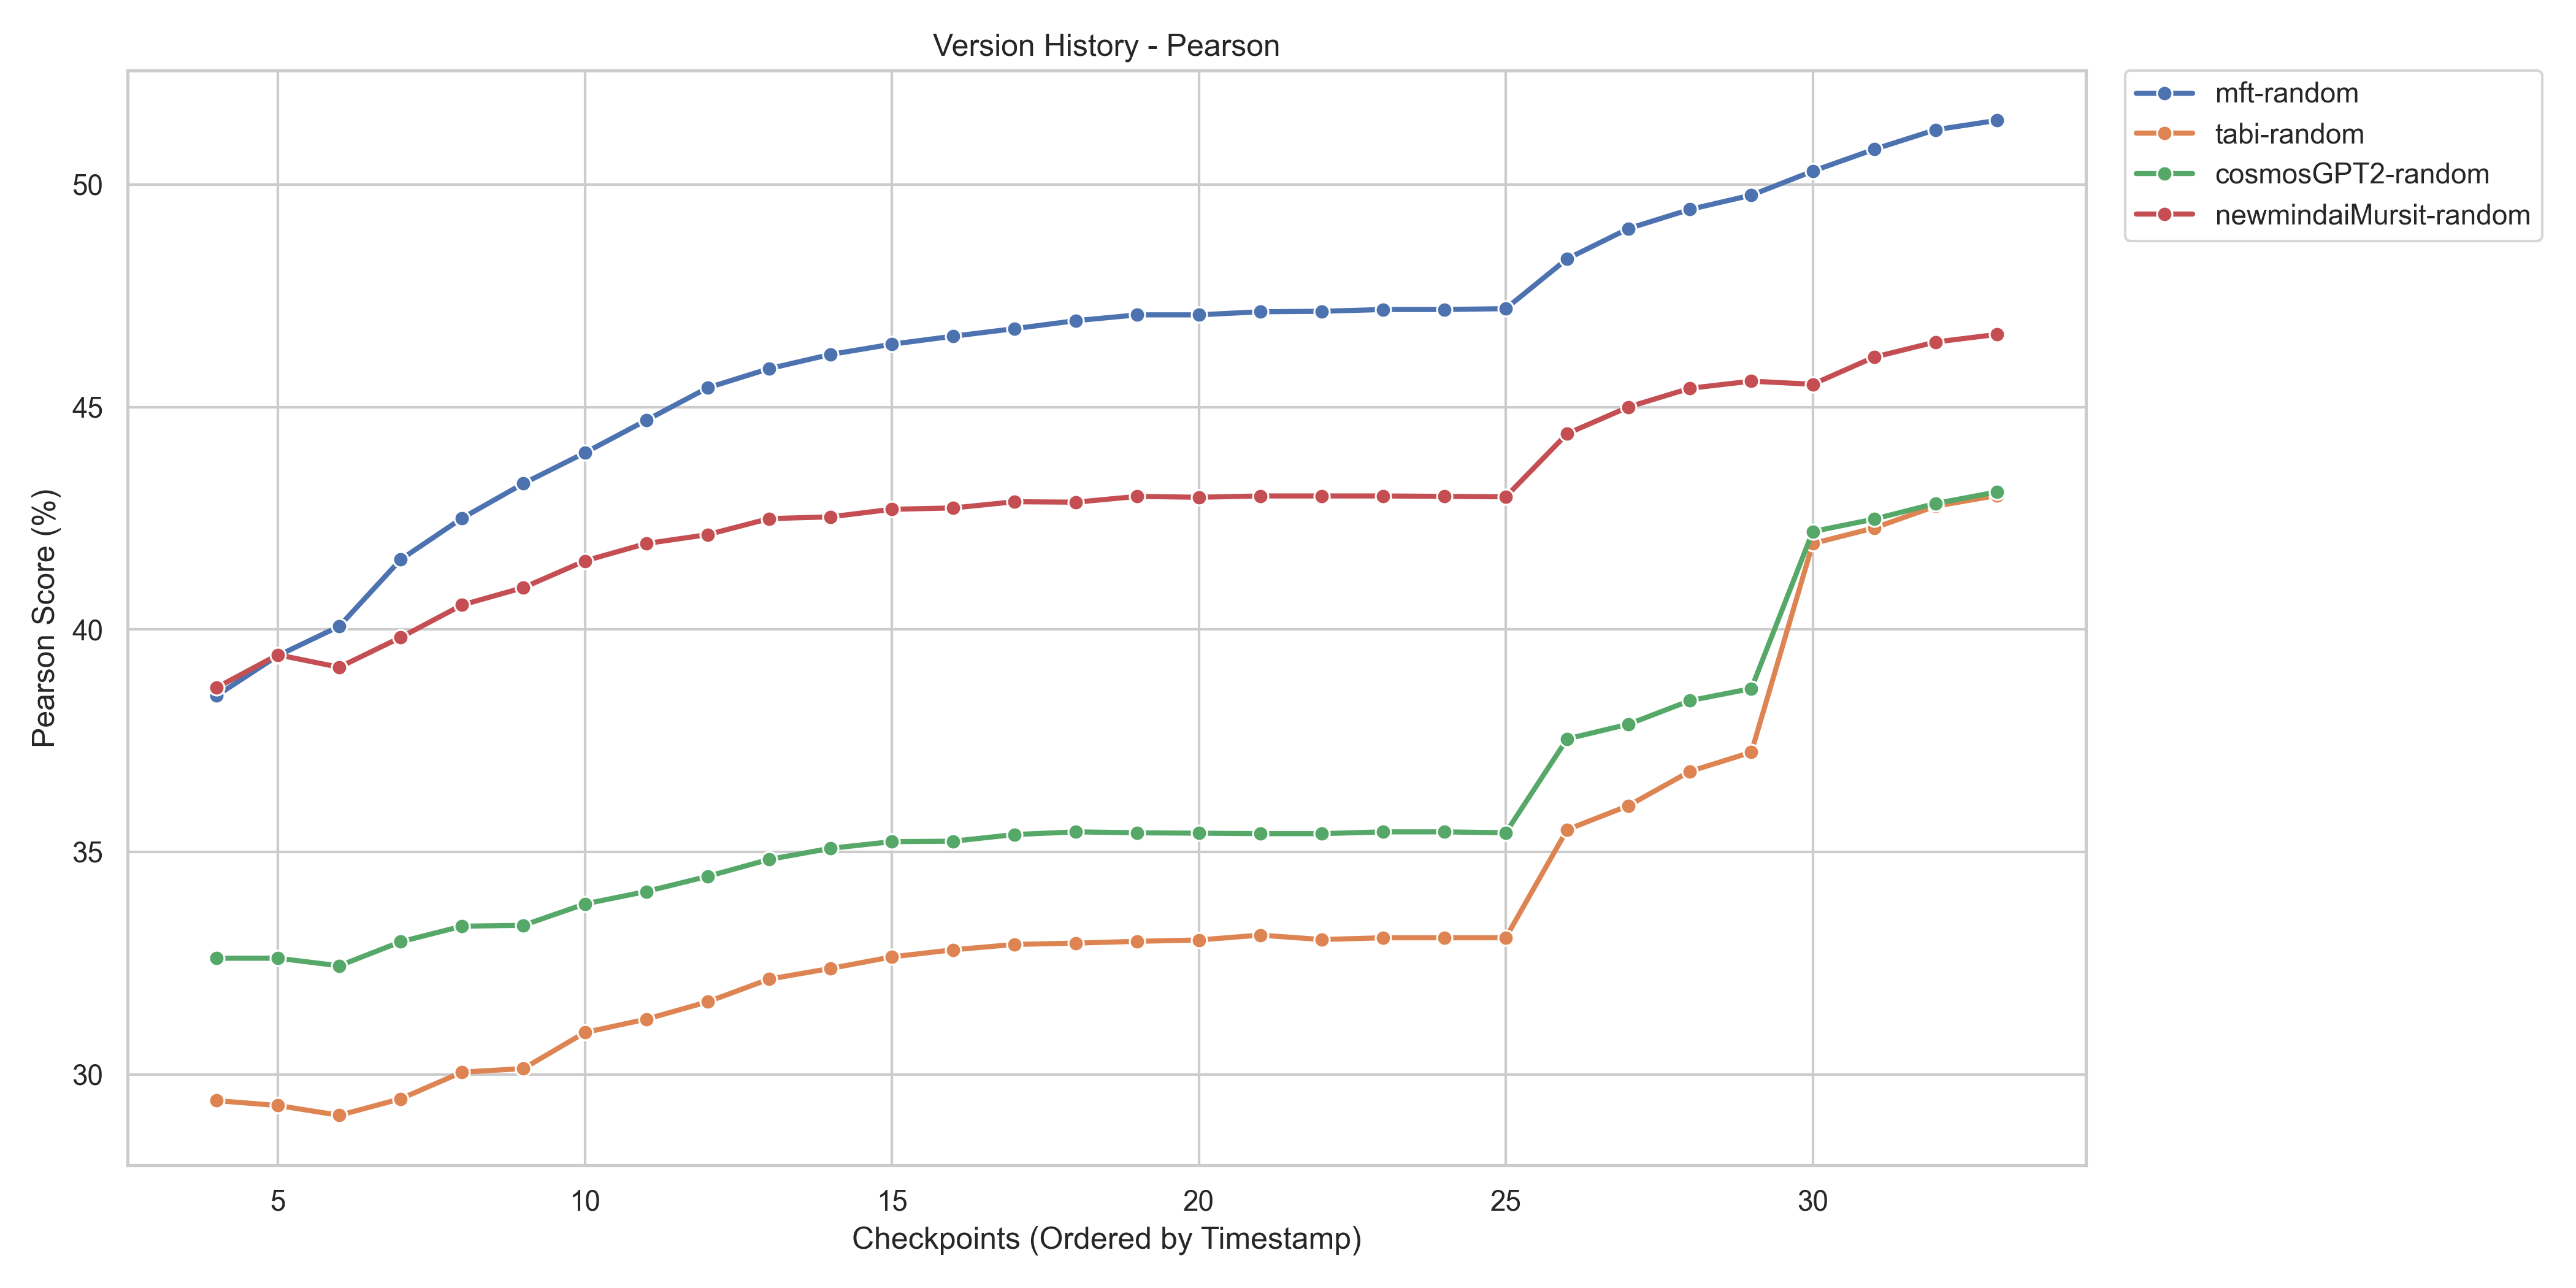
\includegraphics[width=0.85\linewidth]{figures/version_history_pearson.png}
    \caption{Pearson correlation across model revisions.}
    \label{fig:version_history_pearson}
\end{figure}

Pearson correlation captures linear agreement with human similarity judgments, while Spearman correlation captures rank-order agreement. Reporting both is important in STS, since models may preserve relative similarity ordering even when the mapping is not perfectly linear, and conversely small linear gains may not reflect better ranking behavior.

In our version tracking, both correlations show the same qualitative trend: TurkishTokenizer remains ahead of the strongest baselines across revisions, indicating that the downstream improvement is stable rather than a single-run artifact. Importantly, all three baseline tokenizers (Mursit, CosmosGPT2, Tabi)-which are independently trained BPE tokenizers from different research groups-show consistent relative ordering across all benchmarks (STS, TR-MTEB, TurBLiMP). This cross-tokenizer consistency provides strong evidence that the observed performance differences reflect genuine tokenizer-induced inductive bias rather than random initialization variance: it is statistically implausible for TurkishTokenizer to outperform three independent baselines by chance across multiple evaluation dimensions. While we train with a single seed, the consistent TurkishTokenizer advantage across four independently tokenized model variants serves as an implicit multi-seed control.

On the comprehensive TR-MTEB suite~\cite{baysan-gungor-2025-tr}, which covers retrieval, classification, clustering, and pair classification tasks, the TurkishTokenizer-based model achieves the strongest overall average among the compared random-initialized baselines.

\begin{figure}[H]
    \centering
    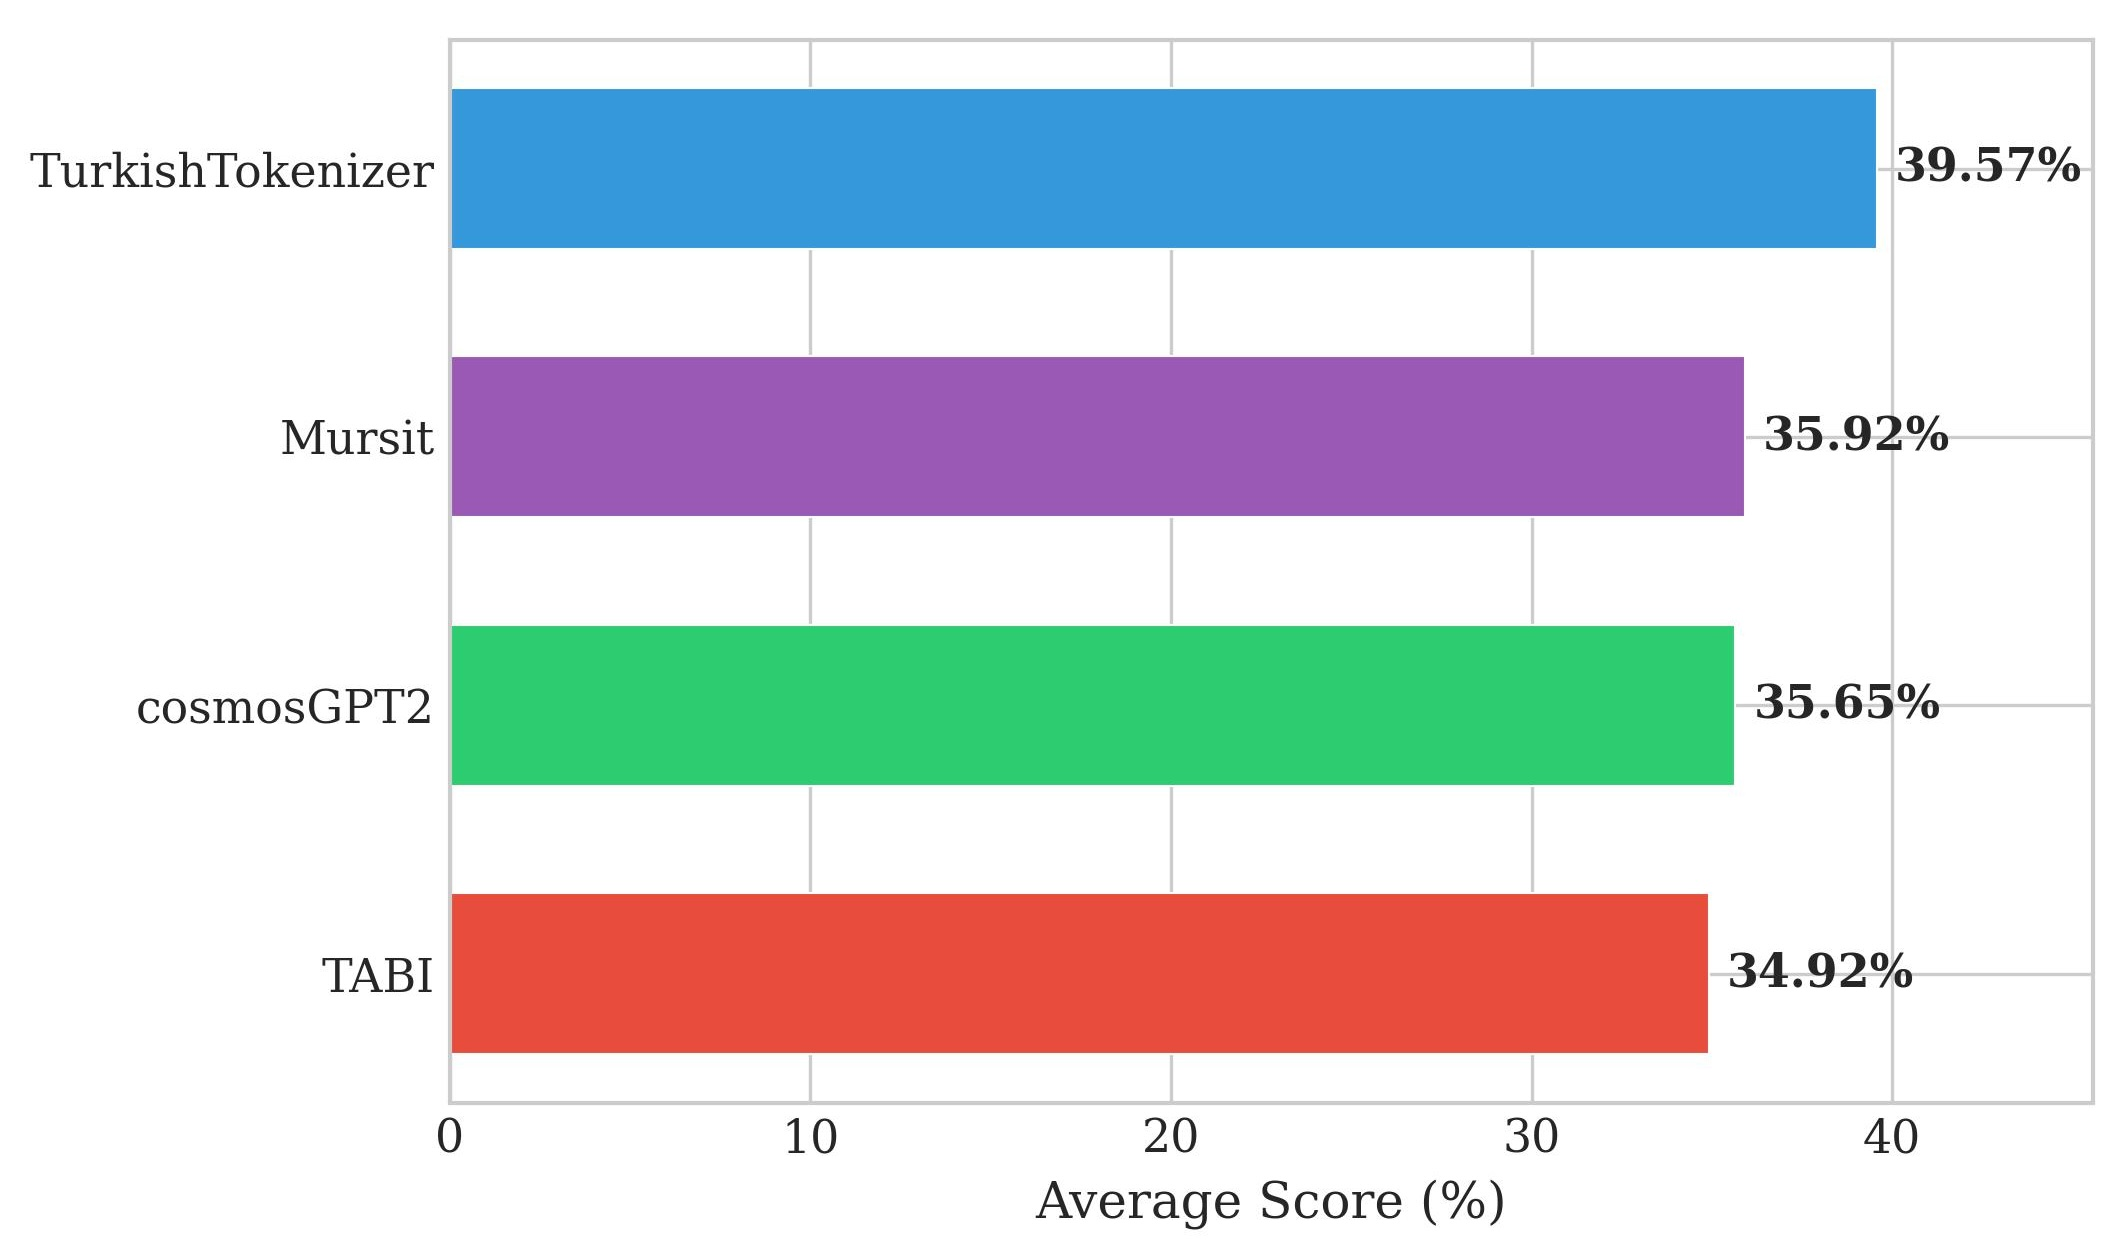
\includegraphics[width=0.92\linewidth]{figures/mteb_comparison.jpg}
    \caption{TR-MTEB overall comparison.}
    \label{fig:mteb_average}
\end{figure}

Figure~\ref{fig:mteb_average} aggregates performance across all evaluated TR-MTEB tasks into a single overall score per model. To make this comparison more interpretable, we next break results down by category (Table~\ref{tab:mteb_category_averages}) and by individual task (Table~\ref{tab:mteb_detailed}), which helps identify where morphology-aware tokenization provides the largest gains and where differences are smaller.

\begin{table}[H]
\centering
\caption{TR-MTEB category averages.}
\label{tab:mteb_category_averages}
\begin{tabular}{lrrrr}
\toprule
\textbf{Category} & \textbf{TurkishTokenizer} & \textbf{Mursit} & \textbf{CosmosGPT2} & \textbf{Tabi} \\
\midrule
BitextMining & \textbf{1.89} & 1.63 & 1.43 & 1.49 \\
Classification & \textbf{59.03} & 57.63 & 57.86 & 57.57 \\
Clustering & 65.49 & 65.83 & \textbf{67.06} & 65.18 \\
Other & \textbf{4.59} & 2.71 & 2.03 & 2.04 \\
Pair Classification & \textbf{50.49} & 47.40 & 48.50 & 47.17 \\
Retrieval & \textbf{30.43} & 23.27 & 22.43 & 21.17 \\
STS & \textbf{50.04} & 45.73 & 42.14 & 42.54 \\
\bottomrule
\end{tabular}
\end{table}

Category-level means summarize broad regimes (retrieval vs.\ classification vs.\ STS), but they can hide task-specific effects. For completeness and transparency, Table~\ref{tab:mteb_detailed} reports the full task-level breakdown.

\begin{table}[H]
\centering
\caption{Detailed TR-MTEB task-level performance.}
\label{tab:mteb_detailed}
\resizebox{\linewidth}{!}{
\begin{tabular}{lrrrr}
\toprule
\textbf{Task} & \textbf{TurkishTokenizer} & \textbf{Mursit} & \textbf{CosmosGPT2} & \textbf{Tabi} \\
\midrule
\multicolumn{5}{l}{\textit{BitextMining}} \\
WMT16BitextMining & \textbf{1.89} & 1.63 & 1.43 & 1.49 \\
\multicolumn{5}{l}{\textit{Classification}} \\
THYSentimentClassification & 51.53 & \textbf{53.08} & 51.18 & 47.17 \\
TSTimelineNewsCategoryClassification & \textbf{50.19} & 45.65 & 44.35 & 44.67 \\
Turkish75NewsClassification & 78.00 & 72.67 & 77.33 & \textbf{80.00} \\
TurkishIronyClassification & 49.50 & 52.67 & 51.17 & \textbf{53.08} \\
TurkishMovieSentimentClassification & \textbf{55.09} & 54.82 & 53.45 & 54.42 \\
TurkishNewsCategoryClassification & \textbf{85.28} & 82.40 & 84.00 & 81.48 \\
TurkishOffensiveLanguageClassification & 49.59 & 48.41 & \textbf{50.31} & 48.65 \\
TurkishProductSentimentClassification & \textbf{53.09} & 51.32 & 51.10 & 51.09 \\
\multicolumn{5}{l}{\textit{Clustering}} \\
TurkishColumnWritingClustering & 65.49 & 65.83 & \textbf{67.06} & 65.18 \\
\multicolumn{5}{l}{\textit{Other}} \\
ArguAnaTR & \textbf{7.28} & 3.77 & 3.35 & 2.67 \\
FiQA2018TR & \textbf{5.79} & 3.95 & 2.42 & 2.81 \\
SCIDOCSTR & \textbf{0.70} & 0.40 & 0.33 & 0.65 \\
\multicolumn{5}{l}{\textit{Pair Classification}} \\
MnliTr & \textbf{48.38} & 46.32 & 46.23 & 45.16 \\
SnliTr & \textbf{45.33} & 41.47 & 41.11 & 40.35 \\
XNLI & 57.76 & 54.41 & \textbf{58.17} & 55.99 \\
\multicolumn{5}{l}{\textit{Retrieval}} \\
CQADupstackGamingRetrievalTR & \textbf{13.17} & 8.75 & 8.24 & 7.27 \\
MSMarcoTRRetrieval & \textbf{15.83} & 8.37 & 7.52 & 7.11 \\
NFCorpusTR & \textbf{1.32} & 0.59 & 0.51 & 0.24 \\
QuoraRetrievalTR & \textbf{63.84} & 52.20 & 49.02 & 47.46 \\
SciFactTR & \textbf{23.97} & 21.19 & 19.86 & 17.34 \\
SquadTRRetrieval & \textbf{18.74} & 10.69 & 9.94 & 8.78 \\
TQuadRetrieval & \textbf{46.92} & 35.43 & 33.81 & 34.96 \\
TurkishAbstractCorpusClustering & \textbf{47.83} & 43.63 & 44.24 & 41.20 \\
XQuADRetrieval & \textbf{42.27} & 28.55 & 28.69 & 26.19 \\
\multicolumn{5}{l}{\textit{STS}} \\
STSbTR & \textbf{50.04} & 45.73 & 42.14 & 42.54 \\
\bottomrule
\end{tabular}
}
\end{table}

As shown in Table \ref{tab:mteb_detailed}, the TurkishTokenizer-based model achieved an average score of \textbf{39.57\%} across 26 TR-MTEB tasks, surpassing Mursit (35.92\%), CosmosGPT2 (35.65\%), and Tabi (34.92\%). Analyzing performance by category reveals distinct trade-offs. TurkishTokenizer demonstrates substantial advantages in \textit{STS} and \textit{Retrieval} tasks (e.g., TQuadRetrieval: 46.92\% vs 34.96\% for Tabi), which aligns with our hypothesis that morphology-aware segmentation improves the semantic quality of embeddings for similarity and search. At the same time, the Tabi baseline remains competitive or superior in specific \textit{Classification} tasks (e.g., Turkish75NewsClassification: 80.00\% vs 78.00\% for TurkishTokenizer), suggesting that different tokenization priors can favor different downstream regimes even under matched architecture and training protocol.

While TR-MTEB provides broad downstream coverage, it does not isolate controlled grammatical manipulations. We therefore complement it with TurBLiMP, which probes specific linguistic phenomena via minimal pairs.


TurBLiMP provides Turkish minimal pairs designed to probe specific linguistic phenomena (e.g., agreement, scrambling, nominalization) \cite{basar_turblimp_2025}. Since our models are sentence embedding encoders (rather than generative language models), we evaluate a centroid-based acceptability proxy: for each phenomenon file, we compute the centroid of the grammatical sentence embeddings, score each sentence by cosine similarity to this centroid, and count a minimal pair as correct if the grammatical sentence receives a higher score than its ungrammatical counterpart. We report the resulting pairwise accuracy per phenomenon (in \%) in Table~\ref{tab:turblimp_detailed}. Following the visualization convention used in the TurBLiMP paper, cell background colors indicate relative performance, ranging from lower (red) to higher (green).

\begin{table}[H]
\centering
\caption{TurBLiMP centroid-based pairwise accuracy by linguistic phenomenon.}
\label{tab:turblimp_detailed}
\resizebox{\linewidth}{!}{
\begin{tabular}{lrrrr}
\toprule
 & TurkishTokenizer & Mursit & CosmosGPT2 & Tabi \\
\midrule
Anaphor Agreement & \cellcolor[RGB]{243,202,95} \textbf{52.3} & \cellcolor[RGB]{255,194,97} 48.6 & \cellcolor[RGB]{255,198,99} 49.6 & \cellcolor[RGB]{255,198,99} 49.6 \\
Argument Str. Tran. & \cellcolor[RGB]{255,189,94} 47.4 & \cellcolor[RGB]{231,205,90} 54.7 & \cellcolor[RGB]{219,207,86} \textbf{57.0} & \cellcolor[RGB]{222,206,87} 56.3 \\
Argument Str. Ditr. & \cellcolor[RGB]{249,201,98} 51.0 & \cellcolor[RGB]{255,145,72} 36.4 & \cellcolor[RGB]{207,210,81} \textbf{59.3} & \cellcolor[RGB]{247,201,97} 51.4 \\
Binding & \cellcolor[RGB]{67,240,26} \textbf{86.7} & \cellcolor[RGB]{149,222,58} 70.7 & \cellcolor[RGB]{150,222,59} 70.5 & \cellcolor[RGB]{185,214,72} 63.6 \\
Determiners & \cellcolor[RGB]{1,254,0} \textbf{99.7} & \cellcolor[RGB]{18,250,7} 96.3 & \cellcolor[RGB]{32,247,12} 93.6 & \cellcolor[RGB]{212,209,83} 58.4 \\
Ellipsis & \cellcolor[RGB]{189,214,74} \textbf{62.9} & \cellcolor[RGB]{255,197,98} 49.3 & \cellcolor[RGB]{255,189,94} 47.3 & \cellcolor[RGB]{227,205,89} 55.4 \\
Irregular Forms & \cellcolor[RGB]{230,205,90} \textbf{54.9} & \cellcolor[RGB]{255,130,65} 32.7 & \cellcolor[RGB]{255,133,66} 33.3 & \cellcolor[RGB]{255,183,91} 45.9 \\
Island Effects & \cellcolor[RGB]{35,247,13} \textbf{93.1} & \cellcolor[RGB]{255,199,99} 49.9 & \cellcolor[RGB]{255,142,71} 35.7 & \cellcolor[RGB]{251,200,98} 50.7 \\
Nominalization & \cellcolor[RGB]{255,181,90} 45.4 & \cellcolor[RGB]{248,201,97} 51.2 & \cellcolor[RGB]{246,201,96} 51.7 & \cellcolor[RGB]{244,202,95} \textbf{52.1} \\
NPI Licensing & \cellcolor[RGB]{143,224,56} \textbf{71.9} & \cellcolor[RGB]{255,187,93} 46.8 & \cellcolor[RGB]{255,194,97} 48.7 & \cellcolor[RGB]{255,193,96} 48.3 \\
Passives & \cellcolor[RGB]{255,167,83} 41.9 & \cellcolor[RGB]{232,204,91} 54.4 & \cellcolor[RGB]{255,172,86} 43.1 & \cellcolor[RGB]{196,212,77} \textbf{61.5} \\
Quantifiers & \cellcolor[RGB]{255,102,51} 25.5 & \cellcolor[RGB]{255,179,89} \textbf{44.9} & \cellcolor[RGB]{255,84,42} 21.1 & \cellcolor[RGB]{255,79,39} 19.8 \\
Relative Clauses & \cellcolor[RGB]{255,193,96} 48.4 & \cellcolor[RGB]{255,194,97} 48.7 & \cellcolor[RGB]{247,201,97} \textbf{51.5} & \cellcolor[RGB]{255,197,98} 49.4 \\
Scrambling & \cellcolor[RGB]{208,210,81} \textbf{59.1} & \cellcolor[RGB]{221,207,87} 56.5 & \cellcolor[RGB]{227,205,89} 55.3 & \cellcolor[RGB]{226,206,88} 55.6 \\
Subject Agreement & \cellcolor[RGB]{161,220,63} \textbf{68.4} & \cellcolor[RGB]{219,207,86} 56.9 & \cellcolor[RGB]{228,205,89} 55.1 & \cellcolor[RGB]{199,211,78} 60.8 \\
Suspended Affixation & \cellcolor[RGB]{146,223,57} \textbf{71.2} & \cellcolor[RGB]{255,181,90} 45.4 & \cellcolor[RGB]{255,161,80} 40.4 & \cellcolor[RGB]{255,189,94} 47.3 \\
Model Average & \cellcolor[RGB]{197,212,77} \textbf{61.2} & \cellcolor[RGB]{241,202,94} 52.7 & \cellcolor[RGB]{250,200,98} 50.8 & \cellcolor[RGB]{246,201,96} 51.6 \\
\bottomrule
\end{tabular}

}
\end{table}

Across many categories, TurkishTokenizer improves the separation of grammatical vs.\ ungrammatical minimal pairs under this proxy. A complementary evaluation of true grammatical sensitivity would require scoring minimal pairs with language model likelihood or a supervised acceptability classifier, which we leave for future work.

\FloatBarrier
